\chapter{Experimenteller Aufbau}
\label{sec:auf}
In dieser Bachelorarbeit wird ein Terahertz-Zeitbereichsspektrometer genutzt, 
um die THz-Emissionen verschiedener Kristalle zu bestimmen. 
Der schematische Aufbau des THz-TDS-Systems ist in \autoref{fig:thz-aufbau} zu sehen.
Der Laser, der dem Aufbau zugrunde liegt, ist ein gepulster Titan-Saphir-Laser, welcher Nahinfrarot-Pulse  
mit einer Wiederholrate von $\SI{3000}{\kilo\hertz}$ und einer Pulsdauer von $\SI{30}{fs}$ erzeugt. 
Diese haben eine Zentralwellenlänge von $\SI{808}{nm}$. 
Für den Optischen Aufbau steht eine Leistung von $\SI{500}{\milli\watt}$ zur verfügung.
Der Laserstrahl wird zu Begin mithilfe eines Strahlteilers in einen Pumpstrahl mit $99\%$ der Leistung 
und einen Detektionsstrahl mit $1\%$ der Leistung aufgeteilt. Das ist oben links in \autoref{fig:thz-aufbau} gezeigt. 
Der Pumpstrahl ist im Aufbau grün dargestellt und wird von dem Strahlteiler transmittiert, wobei dieser Pfad in \autoref{sec:pump} näher erläutert wird. 
Der Detektionsstrahl wird im Aufbau orange dargestellt und wird von dem Strahlteiler reflektiert, dieser Pfad wird in \autoref{sec:probe} näher erklärt. 

\begin{figure}
    \centering
    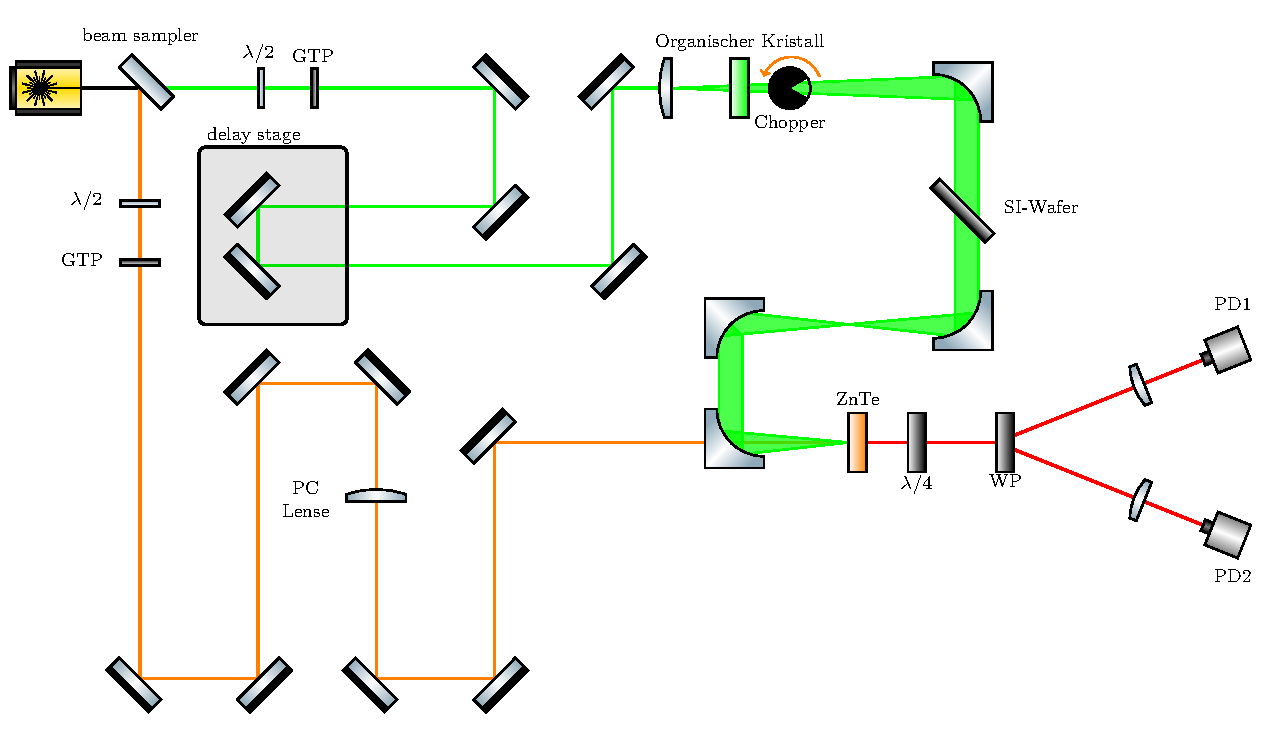
\includegraphics[width=0.8\textwidth]{content/bilder/aufbau.pdf}
    \caption{Schematischer Aufbau von einem Terahertz-Zeitbereichsspektrometers.
    Der grüne Strahl ist der Pump-Strahl, 
    welcher durch den Strahlteiler transmitiert wird und eine Verzögerungsstrecke durchläuft. 
    Anschließend trifft er auf die Generationskristallposition. 
    Hinter dieser wird der Strahl von Parabolspiegeln in die elektrooptische Detektion geleitet. 
    Der Detektionsstrahl, der orange Strahl, wird von dem Strahlteiler reflektiert und 
    wird über mehere Spiegel in die elektrooptische Detektion geführt. 
    }
    \label{fig:thz-aufbau}
\end{figure}

% \section{Terahertz-Zeitbereichsspektroskopie}
% Zu Beginn kommt der Strahl mit einer Leistung von $Platzhalter\,\unit{mW}$ in das Setup. 
% Dies ist in \autoref{fig:thz-aufbau} oben links zu sehen. 
% Im Anschluss trifft dieser Strahl einen Beam splitter, welcher $99\%$ der Intensiität hindurch lässt, 
% was anschließend der Pump-strahl, welcher in der Abbildung grün dargestellt ist, wird in \autoref{sec:pump} weiter beschrieben. 
% Der reflektierte Teil des Strahls, welcher $1\%$ der Leistung des Ausgangsstrahls besitzt, ist 
% dann der Probe-Strahl, welcher in \autoref{fig:thz-aufbau}, Orange dargestellt wird und in \autoref{sec:probe} weiter erläutert wird.



\section{Pump-Strahl}
\label{sec:pump}
Der Pumpstrahl wird zu Beginn durch ein $\lambda/2$-Plättchen, gefolgt von einem Glan-Taylor-Prisma geführt. 
Das $\lambda/2$-Plättchen dreht die Polarisation des Strahls und das Glan-Taylor-Prisma trennt die p- und s-Polarisation 
voneinander. 
Somit lässt sich über diesen Aufbau die Leistung des Strahls einstellen. 
Nach dieser Intensitätseinstellung wird der Pumpstrahl auf die Verzögerungsstrecke geleitet. 
Der aktive Teil dieser Strecke besteht aus einem linearen Positioniertrisch, auf welchem ein Retroreflektor sitzt.
Dieser kann auf einer Länge von $20\,\unit{\milli\meter}$ verfahren werden.
Aufgrund des doppelten Lichtwegs im Retroreflektor entspricht dies einer zeitlichen Verzögerung von $\SI{133}{ps}$.
Auf die Verzögerungsstrecke folgt eine plankonvexe Linse mit einer Brennweite von $100\,\unit{\milli\meter}$. 
Der Fokuspunkt dieser Linse liegt $100\,\unit{\milli\meter}$ vor dem ersten darauffolgenden Parabolspiegel, 
der ebenfalls eine Brennweite von $100\,\unit{\milli\meter}$ besitzt. Somit ist der Strahl nach dem ersten 
Parabolspiegel kollimiert, was in \autoref{fig:thz-aufbau} durch den breiten Strahl gekennzeichnet ist. 
Zwischen dem ersten Parabolspiegel und der Linse befindet sich die Position der Generationskristalle.  
Hinter dem Generationskristall ist ein mechanischer Strahlzerhacker platziert. Dieser moduliert den Strahl mit  
$1500\,\unit{Hz}$, was für die Rauschunterdrückung und Detektion genutzt wird, siehe \autoref{sec:TEOS}.
Anschließend wird der THz-Puls über drei weitere Parabolspiegel geführt.
Zwischen dem ersten und dem zweiten Parabolspiegel ist eine Siliziumscheibe, welche das 
restliche Nahinfrarotlicht, welches nicht in THz-Strahlung umgewandelt wurde, herausfiltert. 
Der vierte und letzte Parabolspiegel fokussiert den Strahl auf den Detektionskristall. 



\section{Detektionsstrahl}
\label{sec:probe}


Zu Beginn durchläuft der Detektionsstrahl ein $\lambda/2$-Plättchen, gefolgt von einem Glan-Taylor-Prisma zur Regulierung 
der Leistung, analog zum Pumpstrahl. 

Der weitere Pfad besteht aus mehreren Spiegeln, um die optische Weglänge zwischen dem Pumpstrahl und dem Detektionsstrahl anzugleichen. 
Mit einer plankonvexen Linse (Brennweite \SI{500}{mm}) wird der Strahl durch ein Loch im vierten Parabolspiegel auf den ZnTe-Kristall fokussiert.
Dort überlappt er räumlich mit dem THz-Puls. Die zeitliche Überlappung kann durch die Verzögerungsstrecke variiert werden. 
Räumlicher Überlapp bedeutet, dass der Fokuspunkt an der Stelle des ZnTe von Pump- und Detektionsstrahl identisch ist. 
Der Punkt des Überlapps wird bestimmt, indem zuerst die Siliziumscheibe entfernt wird, um den Pumpstrahl zu detektieren. 
Anschließend wird an die Stelle des Detektionskristalls eine Kamera platziert, über welche geprüft wird, ob die 
Fokuspunkte übereinander liegen. 
Ist dies nicht der Fall, kann mithilfe der Ausrichtung des letzten Parabolspiegels und des letzten Spiegels 
des Detektionspfades dies korrigiert werden.

Die Messung selber folgt in einer elektrooptischen Detektion, kurz EOS (siehe \autoref{sec:TEOS}). 
Um Streulicht zu vermeiden, wird der Aufbau eingehaust. 
Dazu werden die bancierten Photodioden von verschiedenen Stromversorgungen betrieben. 
Die Dioden werden mit Labornetzgeräten betrieben und auch mit externen Batterien. 
Das gemessene Signal der Photodioden wird anschließend in den Lock-In-Verstärker geleitet und dort zum Auslesen demoduliert.





% bei welchem ein 
% Räumlichen Überlapp mit dem Probe-Strahl erzeugt werden muss. 
% Das bedeutet, dass die beiden Fokuspunkte vom Probe- und Pump-THz-Strahl am selben Ort liegen, dies 
% wird durch eine Kamera und das Verstellen des letzten Parabolspiegels beim THz-Strahl und 
% verstellen des letzten normalen Spiegels des Probe-Strahls gewährleistet. 




%------------Purge Box stuff
% Um systematisch Fehler zu vermindern, wird eine Purge-Box um den Teil des Aufbaus platziert 
% in welchem THz-Strahlung propagiert. 
% Die Purge-Box wird eingerichtet, da THz-Strahlung mit den Wassermolekülen in der Luft interagiert. 
% Diese Interaktion findet statt, da Wasserdampf scharfe Rotations-Absorptionslinien für THz-Strahlung besitzt. 
% Die Kanten sind sehr schmalbandig, also gelten sie nur für einen kleinen Frequenzbereich. 
% Dies hat eine Verzögerung des THz-Signals zur Folge. 
% Wegen der Schmaalen Bandbreite dieser Resonanz für die dadurch verbundende starke Resonanz 
% zu zeitlich verzögterten gedämpften Nachschwingungen, welche nach dem hauptpuls als 
% Echo in den Messdaten auftreten.
% Dieses Echo fungiert dann nur noch als Rauschen und verschlechtert das Messergebnis. 
% Als Lösung für dieses Problem wird eine Box um den in \autoref{fig:thz-aufbau} zu sehenden Teil platziert. 
% Anschließend wird diese Box mit Trockenluft gefüllt, welche explizit keinen Wasserdampf enthält und so 
% die Interaktion nicht stattdindet. 
% Als Alternative könnte diese Box auch mit Stickstoff gefüllt werden oder in dieser ein Vakuum 
% erzeugt werden, was aber deutlich aufwendiger und unpraktikabler ist.



% Das Elektro-Optische Sampling beginnt mit dem eintreffen des Probe- und Pump-Strahls in den 
% ZnTe Detektionskristall. 
% In diesem Kristall ändert sich durch den so gennanten Pockelseffekt \cite{Kühn2011Nonlinear} 
% der Brechungsindex %$\delta n \propto n^3 r E_\text{THz}(t)$% 
% dabei ist wichtig, dass der Probe puls extrem kurz im fs gegenüber dem Pump THz Puls im ps bereich ist 
% und somit immer nur einen Moment des THz Puls abtastet wie in \autoref{fig:thz-puls} zu sehen ist. 
% Die Verschiebung ist wie schon erwäht durch die Delay-station erreichbar. 
% Die Änderung des Brechungsindex hat zu folge, dass durch ein bestimmte drehung des Kristalls 
% diese Doppelbrechend wirkt, was bedeutet, dass der Senktrechte und horizontale teil des stahls 
% unterschiedlich gebrochen werden. 
% Durch diese Doppelbrechung entsteht eine kleine Phasenverzögerung und der vorher Linear 
% Polarisierte Stahl wird zu einem elliptsch polarisertem strahl.
% Anschließend trifft dieser strahl die $\lambda/4$ Platte welchen diesen Elliptsch polarisierten strahl 
% weiter dreht und zu einem nahzu Circulär Polarisiertem Strahl macht. Dieses verhalten entsteht 
% dadurch, dass die $\lambda/4$ Platte eine richtung der Polarisation um ein Viertel der Wellenlänge 
% Verzögert und sich daraus bei einem Perfekt Linearpolarisiertem Stahl ein Circulärpolarisirter 
% Strahl ergibt. Da hier aber ein Elliptischer Strahl vorligt wird der Strahl nach der $\lambda/4 $ Platte 
% nicht perfekt Zirkular sondern elliptsch Polarisiert. 
% Dannach trifft dieser Strahl auf einen Wollaston Prisma welcher den Strahl Räumlich in 
% seine Senkrechte und Waagerechte Polarisation aufteilt, wenn der Strahl ein perfekt 
% Zirkulär Polarisierter Strahl wäre, wären die zwei Resultierenden Strahlen exakt identisch 
% doch durch den THz-Strahl ist hier nun eine leicht elliptsche Polarisation vorhanden. 
% Das hat zufolge, dass ein kleiner Intenistäts unterschied in den beiden Strahlen exisitiert. 
% Diese beiden Strahlen werden dannach durch zwei Photodioden gemessen und verstärkt. 
% Durch diese zwei signale lässt sich dann die differenz also das wirklichen THz-Signal berechnen. 
% Anschließend wird das signal in den Lock-In Verstärker geleitet in welchem das Signal 
% auf die eingestellte frequenz des Choppers demoduliert wird. 
% Das bedeutet die SIgnale die die selbe frequenz wie der Chopper haben werden verstärkt und 
% diese Restlichen mithilfe eines Tiefpassfilters unterdrückt. 
% Dazu werden diese Signale die die Selber frequenz haben über viele Perioden Gemittelt um 
% das Rauschen weiter zu vermindern.


% \begin{figure}
%     \centering
%     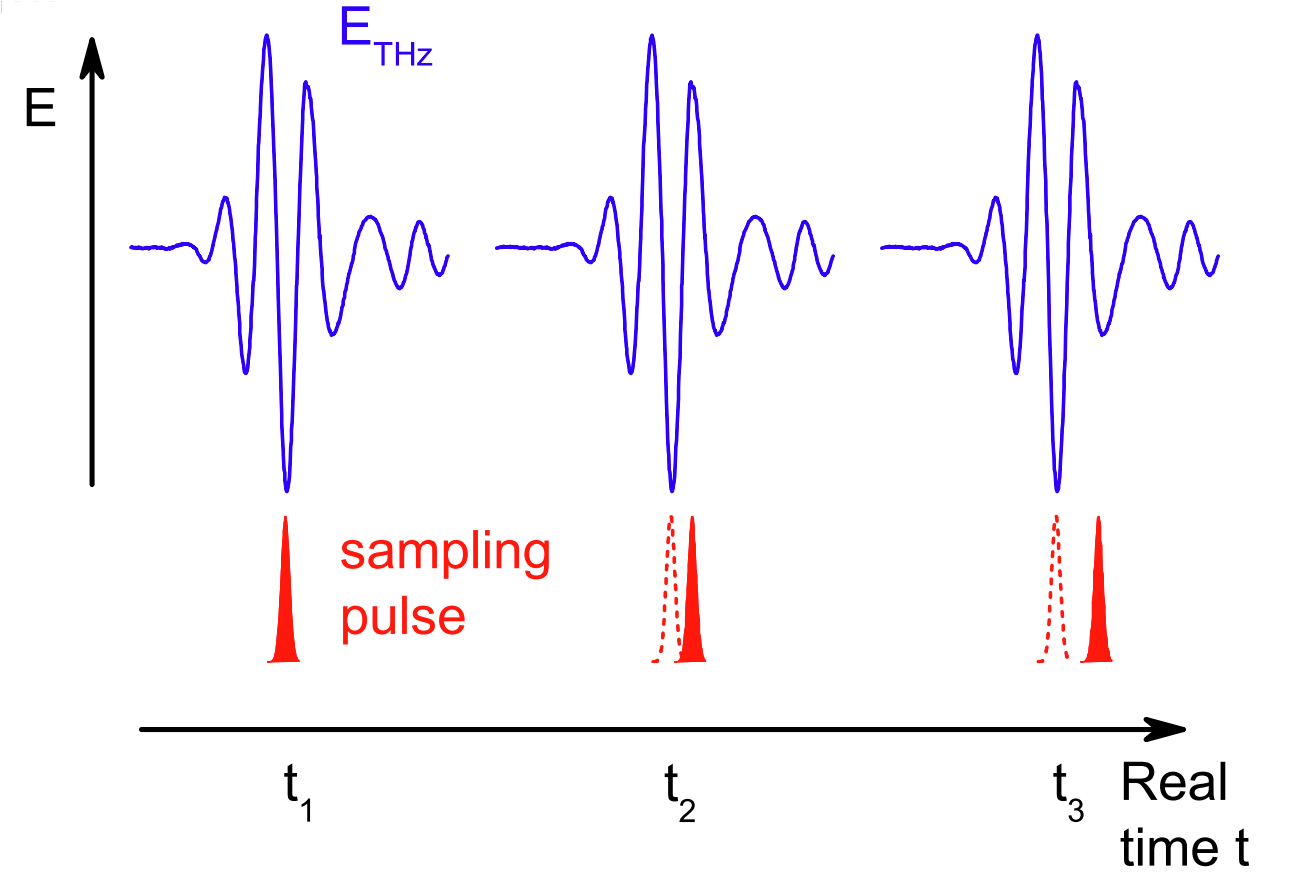
\includegraphics[width=0.8\textwidth]{content/bilder/thz_puls.png}
%     \caption{THz-Puls mit dem Samplingpuls der Abtastend über den THz-Puls fährt durch 
%     die verschiebung der Delay-station\,\cite{Kühn2011Nonlinear}.}
%     \label{fig:thz-puls}
% \end{figure}
